\documentclass[a4paper,11pt]{article}
\usepackage[margin=1in]{geometry}
\usepackage{tikz,tkz-graph,graphicx}
\usepackage{xcolor}
\usetikzlibrary{arrows.meta,positioning,shapes,chains,calc}

\definecolor{lightOrange}{rgb}{0.9921875,0.890625,0.69921875}
\definecolor{darkOrange}{rgb}{0.96875,0.64453125,0.33203125}
\definecolor{skyBlue}{rgb}{0.66796875,0.875,0.97265625}

\newcommand{\listNode}[2]{\node[list,on chain] (#1){\nodepart{second} #2};}
\newcommand{\listHead}[1]{\node[listHead,on chain] (#1) {};} 
\newcommand{\listNil}{\node[listNil,on chain] (nil) {$L. nil$};}
\tikzset{
	every state/.style={
		fill=lightOrange,
		draw=darkOrange,
		inner sep = 0pt,
		minimum size = 5ex 
}
}
\tikzset{
	VertexStyle/.style={
		shape        = circle,
		color        = darkOrange,
		fill         = lightOrange,
		inner sep    = 2pt,
		outer sep    = 0pt,
		minimum size = 12pt,
		text         = black,
		draw
	}
}
\tikzset{
	list/.style={
		rectangle split,
		rectangle split parts=3,
		draw,
		rectangle split horizontal,
		minimum size=18,
		inner sep=6pt,
		fill=lightOrange,
		text=black
	}
}
\tikzset{
	listHead/.style={
		rectangle split,
		rectangle split parts=3,
		draw,
		rectangle split horizontal,
		minimum size=18,
		inner sep=5pt,
		fill=skyBlue,
		text=black
	}
}

\tikzset{
	listNil/.style={
		rectangle split,
		rectangle split parts=2,
		rectangle split horizontal,
		minimum size=18,
		inner sep=5pt,
	}
}

\begin{document}

\section*{Picture}
\begin{figure}[h]
	\centering
	\includegraphics[width=0.7\textwidth]{./3.png}
\end{figure}

\section*{PDF}
\begin{figure}[th]
\centering
\begin{enumerate}
\item
		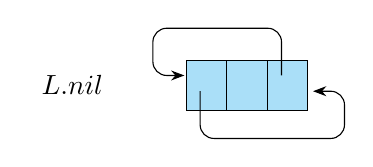
\begin{tikzpicture}[>=Stealth, start chain, node distance=10pt]
		\listNil
		\listHead{head}
		\draw[rounded corners=5pt,->]
		(head.one) -- ++ (0,-0.6)
		-- ($(head.three)+(0.8,-0.6)$)
		-- ++ (0,0.6)
		-- ++ (-0.4,0);
		\draw[rounded corners=5pt,->]
		($(head.three)+(0,0.2)$) -- ++ (0,0.6)
		-- ($(head.one)+(-0.6,0.8)$)
		-- ++(0,-0.6)
		-- ++(0.4,0);
		\end{tikzpicture}
\item
		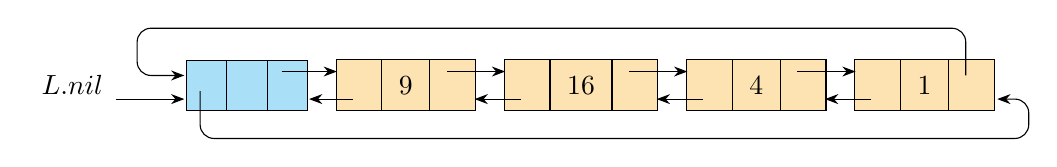
\begin{tikzpicture}[>=Stealth, start chain, node distance=10pt]
		\listNil
		\listHead{head}
		\foreach \Label in {9,16,4,1}
				\listNode{\Label}{$\Label$}
		;

		\foreach \left/\right in {head/9, 9/16, 16/4, 4/1}{%
				\path[->] ($(\left.three)+(0,0.25)$) edge ($(\right.one)+(-0.2,0.25)$);%
				\path[->] ($(\right.one)+(0,-0.1)$) edge ($(\left.three)+(0.35,-0.1)$);%
		}
		\path[->] ($(nil.two)+(-0.2,-0.1)$) edge
		($(head.one)+(-0.2,-0.1)$);%

		\draw[->, rounded corners=5pt] (head.one) -- ++ (0,-0.6)
		-- ($(1.three)+(0.8,-0.6)$) -- ($(1.three)+(0.8,-0.1)$)
		-- ($(1.three)+(0.4,-0.1)$);

		\draw[->, rounded corners=5pt]
		($(1.three)+(0,0.2)$) -- ++ (0,0.6)
		-- ($(head.one)+(-0.8,0.8)$)
		-- ++(0,-0.6)
		-- ++(0.6,0);
		\end{tikzpicture}

\item
		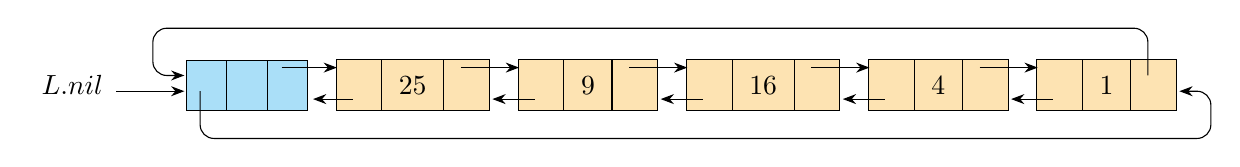
\begin{tikzpicture}[>=Stealth, node distance=10pt, start chain]
		\listNil
		\listHead{head}
		\foreach \Label in {25, 9, 16, 4, 1}{
				\listNode{\Label}{$\Label$}
		}
		\foreach \left/\right in {head/25, 25/9, 9/16, 16/4, 4/1}{
				\draw[->]
				($(\left.three)+(0,0.3)$) -- ($(\right.one)+(-0.2,0.3)$);
				\draw[<-]
				($(\left.three)+(0.4,-0.1)$) -- ($(\right.one)+(0,-0.1)$);
		}
		\draw[->, rounded corners=5pt]
		(head.one) -- ++ (0,-0.6)
		-- ($(1.three)+(0.8,-0.6)$)
		-- ++ (0,0.6)
		-- ++ (-0.4,0);
		\draw[->, rounded corners=5pt]
		($(1.three)+(0,0.2)$)
		-- ++ (0,0.6)
		-- ($(head.one)+(-0.6,0.8)$)
		-- ++ (0,-0.6)
		-- ++ (0.4,0);
		\draw[->] ($(nil.two)+(-0.2,0)$) -- ($(head.one)+(-0.2,0)$);
		\end{tikzpicture}
\item
		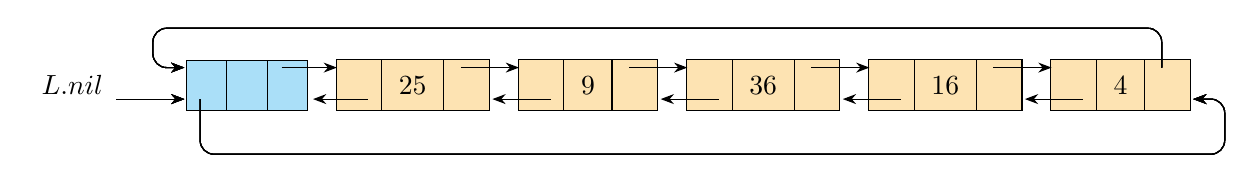
\begin{tikzpicture}[>=Stealth, node distance=10pt, start chain]
		\listNil
		\listHead{head}

		\foreach \Label in {25, 9, 36, 16, 4}{
				\listNode{\Label}{$\Label$}
		}

		\foreach \left/\right in {head/25, 25/9, 9/36, 36/16, 16/4}{
				\draw[->]
				($(\left.three)+(0,0.3)$) -- ($(\right.one)+(-0.2,0.3)$);
				\draw[<-]
				($(\left.three)+(0.4,-0.1)$) -- ($(\right.one)+(0.2,-0.1)$);
				\draw[->, rounded corners=5pt]
				($(head.one)+(0,-0.1)$)
				-- ++ (0,-0.7)
				-- ($(4.three)+(0.8,-0.8)$)
				-- ++ (0,0.7)
				-- ++(-0.4,0);
				\draw[->, rounded corners=5pt]
				($(4.three)+(0,0.3)$)
				-- ++ (0,0.5)
				-- ($(head.one)+(-0.6,0.8)$)
				-- ++ (0,-0.5)
				-- ++ (0.4,0);
				\draw[->]
				($(nil.second)+(-0.2,-0.1)$) -- ($(head.one)+(-0.2,-0.1)$);
		}
		\end{tikzpicture}
\end{enumerate}  
\end{figure}

\end{document}
